% =============================================================================
% best_equipo_04.tex - El ensamble óptimo (m24_ens_optimo) frente al test de Chapinero
% Problem Set 3, Big Data y Machine Learning, Universidad de los Andes, 2026-2
% Figuras y cifras: code/95b_presentacion_best.R (desde el main: Rscript code/00_main.R --solo=95b_presentacion_best.R),
% que las deja en output/{figures,tables}/03_presentacion/best_equipo_04/ y compila este archivo con latexmk.
% Compilar desde esta carpeta: latexmk -pdf best_equipo_04.tex
% =============================================================================
\documentclass[aspectratio=169,10pt]{beamer}

\usepackage[T1]{fontenc}
\usepackage[utf8]{inputenc}
\usepackage[spanish,es-noshorthands,es-nodecimaldot,es-tabla]{babel}
\usepackage{newpxtext,newpxmath}        % Palatino: la misma tipografía de las figuras
\usepackage{booktabs,amsmath,graphicx}
\graphicspath{{../../output/figures/03_presentacion/best_equipo_04/}}
\newcommand{\tablas}{../../output/tables/03_presentacion/best_equipo_04}
\input{\tablas/cifras.tex}
\input{\tablas/cifras_vs.tex}   % sección "por qué no funcionaron las variables del Chapinero sintético"

% ---- Estilo sobrio: solo negro y azul ----
\definecolor{tinta}{HTML}{000000}
\definecolor{gris}{HTML}{1F4E9C}       % azul (textos secundarios, viñetas, pie)
\definecolor{grisclaro}{HTML}{A8C0E6}  % azul claro (reglas)
\definecolor{acento}{HTML}{1F4E9C}     % azul fuerte (énfasis)
\usefonttheme{serif}
\setbeamertemplate{navigation symbols}{}
\setbeamercolor{normal text}{fg=tinta,bg=white}
\setbeamercolor{structure}{fg=tinta}
\setbeamercolor{frametitle}{fg=tinta}
\setbeamercolor{alerted text}{fg=acento}
\setbeamercolor{itemize item}{fg=gris}
\setbeamercolor{enumerate item}{fg=tinta}
\setbeamerfont{frametitle}{size=\large}
\setbeamertemplate{itemize item}{\raisebox{.15ex}{\textendash}}
\setbeamertemplate{enumerate item}{\insertenumlabel.}
\setlength{\leftmargini}{1.1em}
\setbeamertemplate{frametitle}{%
  \vspace*{.6em}\insertframetitle\par\vspace{.1em}{\color{grisclaro}\rule{\linewidth}{.4pt}}}
\setbeamertemplate{footline}{%
  \hspace*{1.2em}{\color{gris}\tiny Equipo 04 · El ensamble óptimo frente al test de Chapinero}\hfill
  {\color{gris}\tiny\insertframenumber}\hspace*{1.2em}\vspace*{.7em}}
\setbeamersize{text margin left=1.2em,text margin right=1.2em}

\newcommand{\nota}[1]{\par\vfill{\color{gris}\scriptsize #1\par}\vspace{.2em}}
\newcommand{\M}{\,M}   % millones de pesos
\newcommand{\mensaje}[1]{\par\vspace{.35em}{\color{acento}\rule[.2ex]{.8em}{.6pt}}\enspace\textbf{#1}}

\title{Un Chapinero sintético para predecir precios}
\subtitle{Qué hace, cuánto acierta y dónde falla el ensamble óptimo}
\author{Juan Manuel Lozano \and María José Perez \and Samuel Suárez}
\institute{Big Data y Machine Learning · Universidad de los Andes}
\date{Problem Set 3 · 2026-2}

\begin{document}

% -----------------------------------------------------------------------------
\begin{frame}[plain]
  \vfill
  {\LARGE \inserttitle\par}\vspace{.4em}
  {\large\color{gris}\insertsubtitle\par}\vspace{1.2em}
  {\color{grisclaro}\rule{.55\linewidth}{.4pt}}\par\vspace{.9em}
  Juan Manuel Lozano \quad·\quad María José Perez \quad·\quad Samuel Suárez\par\vspace{.3em}
  {\small\color{gris}Equipo 04 · Big Data y Machine Learning · Universidad de los Andes · 2026-2\par}
  \vfill
  {\small\color{gris}MAE en Kaggle: público \kPubCompleto, privado \kPrivCompleto\par}
  \vspace*{1.5em}
\end{frame}

% -----------------------------------------------------------------------------
\begin{frame}{El test no se parece al train: predecimos un barrio que casi no vimos}
  \begin{columns}[T,onlytextwidth]
    \begin{column}{.28\textwidth}
      \centering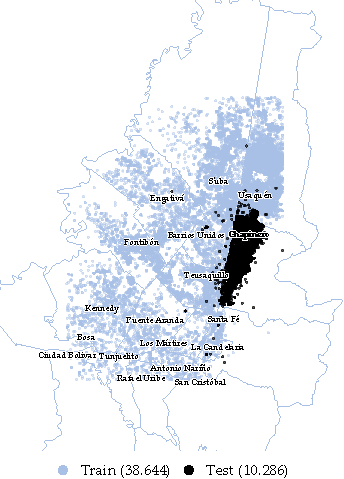
\includegraphics[width=\linewidth]{f01_mapa}
    \end{column}
    \begin{column}{.37\textwidth}
      \vspace{.4em}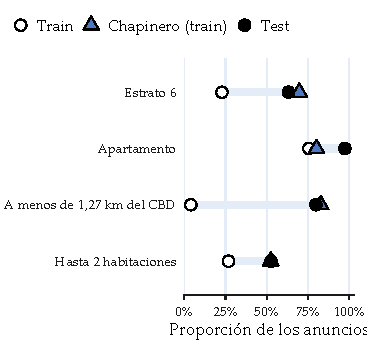
\includegraphics[width=\linewidth]{f02_composicion}
    \end{column}
    \begin{column}{.33\textwidth}
      \small
      \begin{itemize}\setlength{\itemsep}{.4em}
        \item El \pTestChap\ del test está en Chapinero; en el train, Chapinero es apenas el \pTrainChap\ (\nChapTrain\ anuncios).
        \item Estrato 6: \pTrainEstSeis\ del train frente a \pTestEstSeis\ del test.
        \item A menos de 1,27 km de un CBD: \pTrainCBD\ frente a \alert{\pTestCBD}.
      \end{itemize}
      \mensaje{Validar con todo el train responde otra pregunta que la de Kaggle.}
    \end{column}
  \end{columns}
\end{frame}

% -----------------------------------------------------------------------------
\begin{frame}{Chapinero es el mercado más caro y el más homogéneo de la muestra}
  \begin{columns}[T,onlytextwidth]
    \begin{column}{.62\textwidth}
      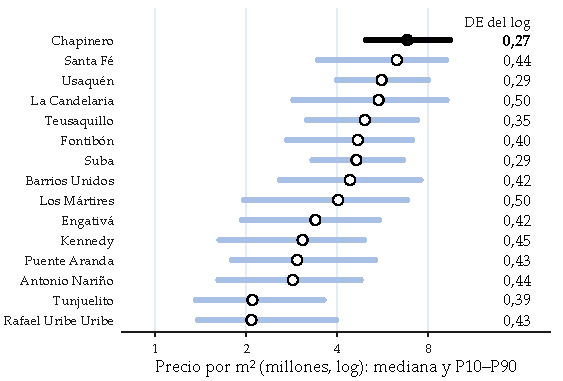
\includegraphics[width=\linewidth]{f03_heterogeneidad}
    \end{column}
    \begin{column}{.35\textwidth}
      \small
      \begin{itemize}\setlength{\itemsep}{.4em}
        \item Mediana de \medPmChap\M\ por m², frente a \medPmTrain\M\ en todo el train.
        \item Menor dispersión de las \nLocHet\ localidades: la DE del log del precio por m² es \sdChap\ (\sdTrain\ en el train).
        \item El test también es compacto: la DE de la distancia al CBD es de \sdCBDTest\ m (\sdCBDTrain\ m en el train).
      \end{itemize}
      \mensaje{El reto no es la varianza dentro del barrio, sino su nivel: es un mercado minoritario en el train.}
    \end{column}
  \end{columns}
\end{frame}

% -----------------------------------------------------------------------------
\begin{frame}{Cómo se construye un Chapinero sintético}
  \small
  \begin{itemize}\setlength{\itemsep}{.3em}
    \item \textbf{Para validar, repesar el train hasta que se parezca al test} (TWCV; Brenning y Suesse, 2026). Los errores fuera de muestra se ponderan por \emph{raking} hasta igualar la composición del test. Los pesos sirven para \emph{evaluar y elegir} hiperparámetros, no para entrenar.
    \item \textbf{Para predecir, un control sintético por anuncio.} Cada inmueble recibe el precio por m² de sus 5 y 20 comparables más cercanos del mismo tipo, ponderados por $1/(d + 30\,\text{m})$.
  \end{itemize}
  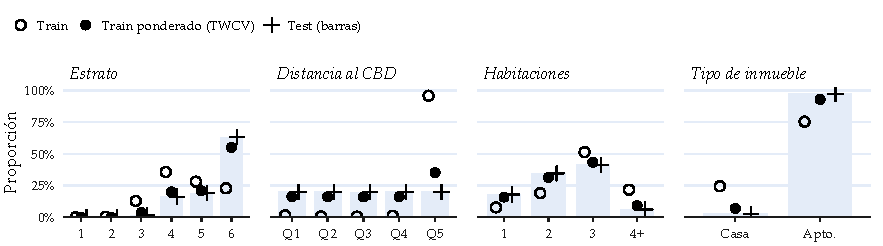
\includegraphics[width=\linewidth]{f04_rebalanceo}
  \nota{Barras: test. Círculos: train sin pesos. Puntos: train con TWCV (pesos encogidos un 20\% hacia la igualdad, como en el artículo).}
\end{frame}

% -----------------------------------------------------------------------------
\begin{frame}{Pero el sintético descansa en pocos anuncios y no ve las distancias del test}
  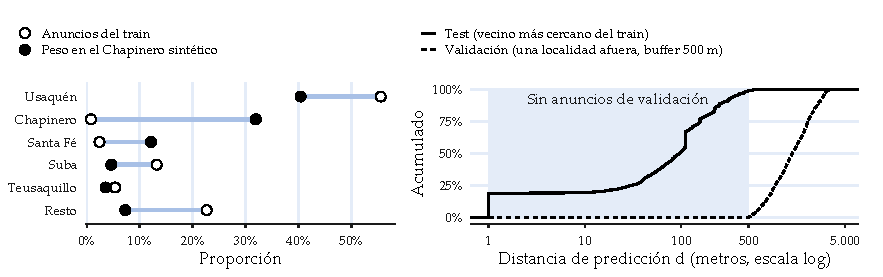
\includegraphics[width=\linewidth]{f05_limites_sintetico}
  \small
  \begin{columns}[T,onlytextwidth]
    \begin{column}{.48\textwidth}
      \begin{itemize}
        \item Tamaño efectivo de la muestra: \alert{\essTWCV\ anuncios} (\pEssTWCV\ del train). Usaquén concentra el \pesoUsaq\ del peso y los \nChapTrain\ anuncios de Chapinero, el \pesoChap.
      \end{itemize}
    \end{column}
    \begin{column}{.48\textwidth}
      \begin{itemize}
        \item En el test, el vecino más cercano del train está a \dMedTest\ m (mediana) y el \pTestDqui\ está a menos de 500 m. En la validación con buffer, \emph{ningún} anuncio lo está.
      \end{itemize}
    \end{column}
  \end{columns}
  \mensaje{Repesar corrige la composición, pero no la geometría del problema.}
\end{frame}

% -----------------------------------------------------------------------------
\begin{frame}{El modelo: un ensamble con pesos óptimos}
  \begin{columns}[T,onlytextwidth]
    \begin{column}{.52\textwidth}
      \small
      \[ \hat p_i = \textstyle\sum_k w_k\,\hat p_{ik}, \qquad w_k \ge 0,\quad \sum_k w_k = 1 \]
      \begin{itemize}\setlength{\itemsep}{.3em}
        \item Con errores aproximadamente normales, $\sigma_k = \sqrt{\pi/2}\,\text{MAE}_k$. La distancia media entre las predicciones de dos modelos identifica la covarianza de sus errores \emph{sin conocer los precios del test}:
        \[ \widehat{\operatorname{Cov}}(e_i,e_j) = \tfrac{1}{2}\big(\sigma_i^2+\sigma_j^2-D_{ij}\big) \]
        \item $w^\ast = \arg\min_w w'\hat\Sigma w$ sobre los 10 modelos con score público.
      \end{itemize}
    \end{column}
    \begin{column}{.45\textwidth}
      \footnotesize\centering\vspace{.6em}
      \begin{tabular}{@{}lrr@{}}
        \toprule
        Componente & Peso & Kaggle (M) \\ \midrule
        Red neuronal STAR & 53,4\% & \kNN \\
        XGBoost con comparables & 39,9\% & \kXGB \\
        Elastic net con texto & 6,6\% & \kEN \\
        Otros 7 candidatos & 0\% & 167--179 \\ \bottomrule
      \end{tabular}
      \par\vspace{1.2em}
      \small\raggedright
      La red y el XGB tienen una correlación de \corNNXGB\ (en log), pero difieren en \difNNXGB\M\ por anuncio: \alert{se equivocan distinto}, y eso es lo que aprovecha el ensamble.\par
    \end{column}
  \end{columns}
\end{frame}

% -----------------------------------------------------------------------------
\begin{frame}{La estimación acertó: \kPub\M\ en el público y \kPriv\M\ en el privado}
  \begin{columns}[T,onlytextwidth]
    \begin{column}{.61\textwidth}
      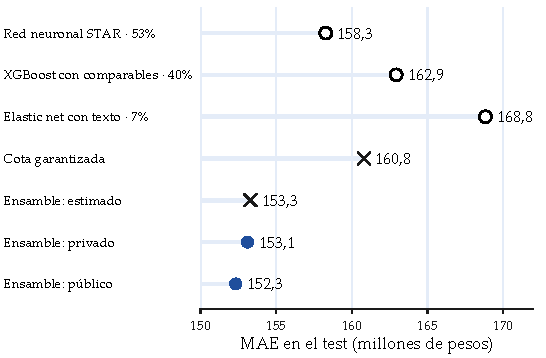
\includegraphics[width=\linewidth]{f06_kaggle}
    \end{column}
    \begin{column}{.36\textwidth}
      \small
      \begin{itemize}\setlength{\itemsep}{.4em}
        \item El método estimó \kEst\M: el resultado quedó prácticamente encima de la estimación y lejos de la cota (\kCota\M).
        \item Mejora en \kGanaNN\M\ al mejor componente (la red neuronal STAR, \kNN\M).
        \item Del público al privado solo empeora \kGapPP\M.
      \end{itemize}
      \mensaje{El ensamble no estaba sobreajustado al leaderboard.}
    \end{column}
  \end{columns}
\end{frame}

% -----------------------------------------------------------------------------
\begin{frame}{Métricas generales: preciso en el centro, débil en las colas}
  \centering\small
  \input{\tablas/metricas.tex}
  \par\vspace{.5em}\raggedright
  \begin{itemize}
    \item El error típico es del 12\%, pero el MAE lo empujan pocos errores grandes. En Chapinero, el modelo \alert{subvalora}.
  \end{itemize}
  \nota{OOF aproximadas: $0{,}534\,\hat p_{\text{red}} + 0{,}399\,\hat p_{\text{XGB}} + 0{,}066\,\hat p_{\text{EN}}$. La red y el elastic net: CV por localidad con buffer. El XGBoost: CV aleatoria, optimista (\maeCompMxxii\M\ frente a \kXGB\M\ en Kaggle).}
\end{frame}

% -----------------------------------------------------------------------------
\begin{frame}{Qué mira el modelo: el tamaño fija el precio; el estrato y los comparables, el m²}
  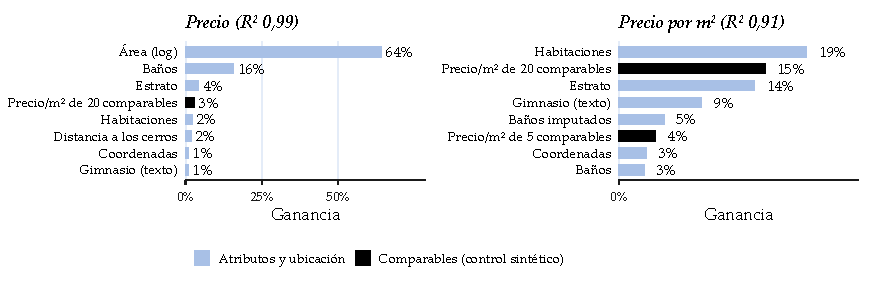
\includegraphics[width=\linewidth]{f07_importancia}
  \small
  \begin{columns}[T,onlytextwidth]
    \begin{column}{.48\textwidth}
      \begin{itemize}
        \item Una red, un XGB y un elastic net no tienen una importancia común. Por eso se ajusta un \emph{modelo sustituto} (XGBoost) que imita la predicción del ensamble en el test.
      \end{itemize}
    \end{column}
    \begin{column}{.48\textwidth}
      \begin{itemize}
        \item El área explica el \gainArea\ del precio, porque dentro de Chapinero la ubicación casi no varía. En el m², los comparables suman el \gainCompM\ y el estrato el \gainEstM.
      \end{itemize}
    \end{column}
  \end{columns}
\end{frame}

% -----------------------------------------------------------------------------
\begin{frame}{Las variables que fijan el valor del m² casi no están en la validación}
  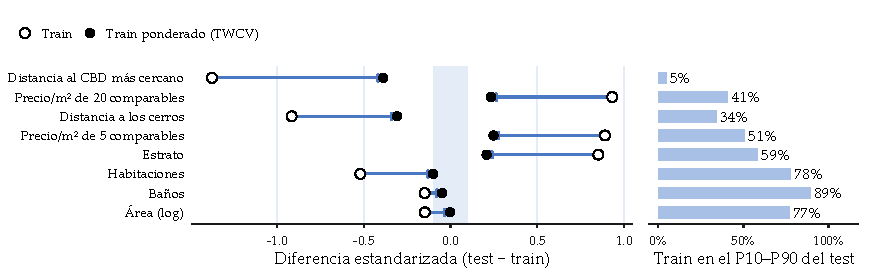
\includegraphics[width=\linewidth]{f08_presencia}
  \small
  \begin{columns}[T,onlytextwidth]
    \begin{column}{.48\textwidth}
      \begin{itemize}
        \item El tamaño y las habitaciones sí están representados. Los comparables, el estrato, los cerros y el CBD se desplazan cerca de una DE; TWCV acorta la brecha, pero no la cierra.
      \end{itemize}
    \end{column}
    \begin{column}{.48\textwidth}
      \begin{itemize}
        \item Solo \alert{\nTrainCaja\ anuncios (\pTrainCaja\ del train)} caen a la vez dentro del rango central (P10--P90) del test en las \nVarsCaja\ variables.
      \end{itemize}
    \end{column}
  \end{columns}
  \nota{Diferencia estandarizada: (media del test $-$ media del train) / DE conjunta. Banda gris: $\pm 0{,}1$, umbral usual de balance.}
\end{frame}

% -----------------------------------------------------------------------------
\begin{frame}{¿Se puede confiar en él para Chapinero? En el centro sí; en el segmento alto, no}
  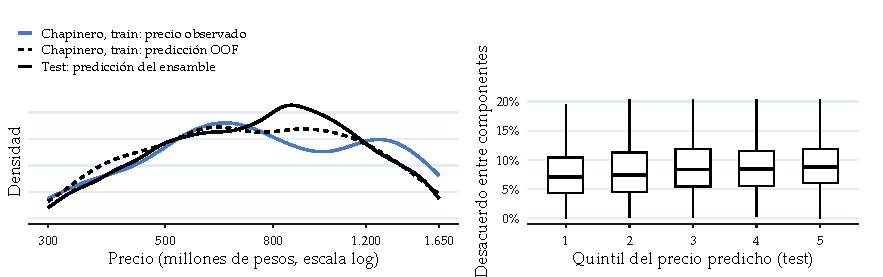
\includegraphics[width=\linewidth]{f11_compresion_test}
  \small
  \begin{columns}[T,onlytextwidth]
    \begin{column}{.48\textwidth}
      \begin{itemize}
        \item La homogeneidad ayuda: en Chapinero (train) el error mediano es del 12\%.
        \item Pero las predicciones están \alert{comprimidas}: el \pObsChapMil\ de Chapinero vale más de 1.200\M; en el test, el modelo solo le asigna eso al \pPredTestMil.
      \end{itemize}
    \end{column}
    \begin{column}{.48\textwidth}
      \begin{itemize}
        \item Los componentes discrepan más justo en los inmuebles más caros (derecha).
      \end{itemize}
      \mensaje{Sirve para valorar la mayor parte del barrio, no su segmento alto.}
    \end{column}
  \end{columns}
\end{frame}

% -----------------------------------------------------------------------------
\begin{frame}{Dónde falla: subvalora los inmuebles caros y sobrevalora los baratos}
  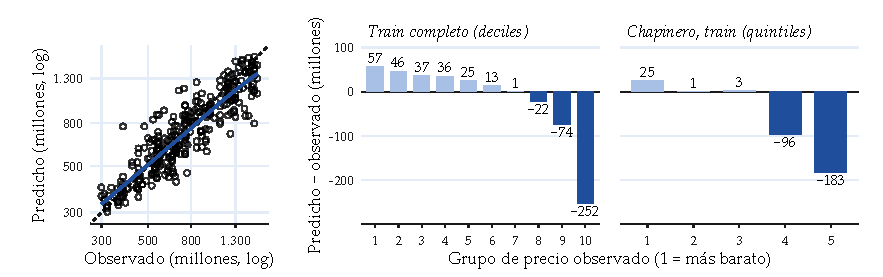
\includegraphics[width=\linewidth]{f10_donde_falla}
  \small
  \begin{columns}[T,onlytextwidth]
    \begin{column}{.48\textwidth}
      \begin{itemize}
        \item Contracción hacia la media: el error promedio (predicho $-$ observado) es de \alert{\sesgoDecTop\M} en el decil más caro y de $+$\sesgoDecBot\M\ en el más barato.
      \end{itemize}
    \end{column}
    \begin{column}{.48\textwidth}
      \begin{itemize}
        \item En Chapinero, el quintil más caro (mediana de \ymedChapTop\M) tiene un sesgo de \sesgoChapTop\M\ por anuncio. Ahí se concentra el error.
      \end{itemize}
    \end{column}
  \end{columns}
\end{frame}

% -----------------------------------------------------------------------------
\begin{frame}{Por qué falla el sintético (1): la validación es más fácil que el test}
  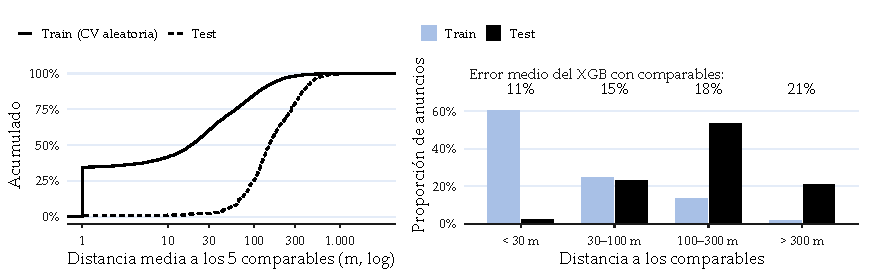
\includegraphics[width=\linewidth]{f09_comparables}
  \small
  \begin{columns}[T,onlytextwidth]
    \begin{column}{.48\textwidth}
      \begin{itemize}
        \item En la CV aleatoria, los comparables de un anuncio del train están a \dCompTrain\ m (mediana), muchas veces en el \emph{mismo edificio}. En el test están a \dCompTest\ m.
      \end{itemize}
    \end{column}
    \begin{column}{.48\textwidth}
      \begin{itemize}
        \item El XGB con comparables se equivoca un \mapeXGBcerca\ con vecinos a menos de 30 m (el \pTrMenosTreinta\ del train) y un \mapeXGBlejos\ entre 100 y 300 m, donde está la mitad del test.
      \end{itemize}
    \end{column}
  \end{columns}
\end{frame}

% -----------------------------------------------------------------------------
\begin{frame}{Por qué falla el sintético (2): corrige la composición, no la falta de soporte}
  \begin{columns}[T,onlytextwidth]
    \begin{column}{.58\textwidth}
      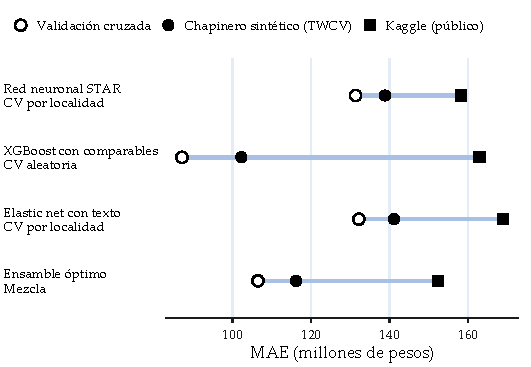
\includegraphics[width=\linewidth]{f12_brecha}
    \end{column}
    \begin{column}{.39\textwidth}
      \small
      \begin{itemize}\setlength{\itemsep}{.35em}
        \item TWCV acerca la validación a Kaggle, pero no llega: en los modelos enviados, el optimismo baja de \sesgoCVloc\M\ a \sesgoCVtw\M\ en promedio.
        \item Brecha entre TWCV y Kaggle: \brechaNN\M\ en la red, \alert{\brechaXGB\M\ en el XGB} y \brechaEns\M\ en el ensamble.
        \item Tres causas: (i) repesar no crea los anuncios caros y céntricos que faltan; (ii) se balancean 5 variables por separado, no su combinación; (iii) la CV de los comparables usa vecinos que el test no tiene.
      \end{itemize}
    \end{column}
  \end{columns}
\end{frame}

% -----------------------------------------------------------------------------
\begin{frame}{Por qué no funcionaron las variables del sintético (1): explican el precio, no el error}
  \begin{center}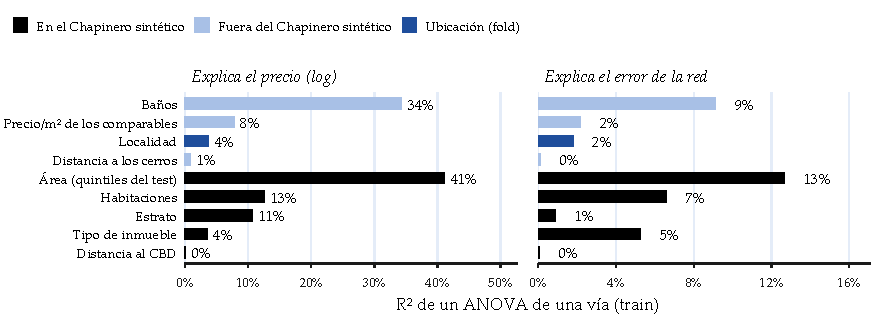
\includegraphics[width=.8\linewidth]{f13_variables_explican}\end{center}
  \small
  \begin{columns}[T,onlytextwidth]
    \begin{column}{.48\textwidth}
      \begin{itemize}
        \item Estrato, tipo, habitaciones, área y distancia al CBD se eligieron porque fijan el precio: juntas explican el \rDosPrecioCinco\ de su varianza (en log).
      \end{itemize}
    \end{column}
    \begin{column}{.48\textwidth}
      \begin{itemize}
        \item Pero explican poco del error de la red: juntas, el \rDosErrCinco; la distancia al CBD, casi nada. Repesar solo cambia el MAE si el error depende de lo que se repesa.
      \end{itemize}
    \end{column}
  \end{columns}
\end{frame}

% -----------------------------------------------------------------------------
\begin{frame}{Por qué no funcionaron (2): el gemelo sintético no tiene el nivel de Chapinero}
  \begin{center}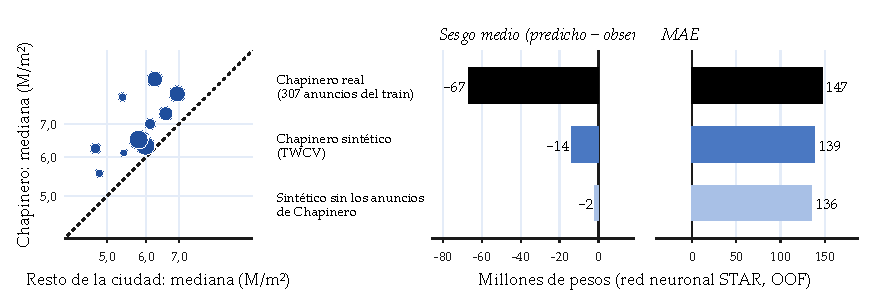
\includegraphics[width=.8\linewidth]{f14_gemelo}\end{center}
  \small
  \begin{columns}[T,onlytextwidth]
    \begin{column}{.48\textwidth}
      \begin{itemize}
        \item Con las mismas 5 variables, un anuncio de Chapinero vale un \alert{\primaChap\ más por m²}; en las \nCeldas\ celdas estrato $\times$ área comparables, Chapinero queda por encima.
      \end{itemize}
    \end{column}
    \begin{column}{.48\textwidth}
      \begin{itemize}
        \item Chapinero pesa solo el \pesoChapSint\ del sintético. La red subvalora Chapinero en \sesgoChapReal\M, pero a su gemelo solo en \sesgoSint\M\ (\sesgoSintSin\M\ sin Chapinero).
      \end{itemize}
      \mensaje{El error es de nivel (ubicación), y las 5 variables no lo ven.}
    \end{column}
  \end{columns}
\end{frame}

% -----------------------------------------------------------------------------
\begin{frame}{Por qué no funcionaron (3): más variables, menos muestra, casi el mismo optimismo}
  \begin{center}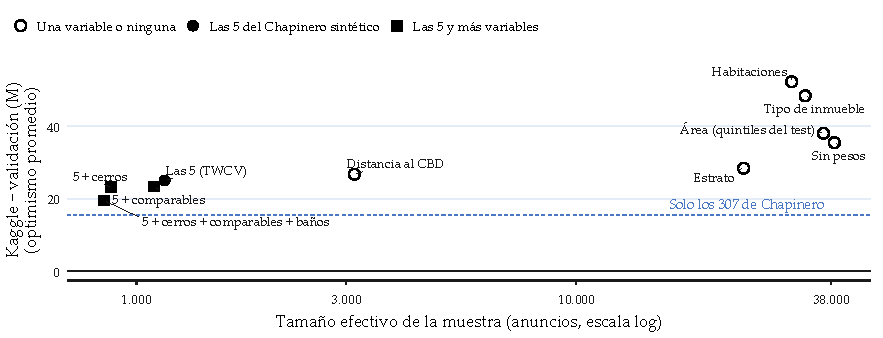
\includegraphics[width=.8\linewidth]{f15_ablacion_pesos}\end{center}
  \small
  \begin{columns}[T,onlytextwidth]
    \begin{column}{.48\textwidth}
      \begin{itemize}
        \item En \nModKaggle\ modelos enviados, la validación sin pesos es \optSinPesos\M\ más optimista que Kaggle; con las 5, \optCinco\M. Casi toda la mejora viene de la distancia al CBD (\optUnaMejor\M\ sola).
      \end{itemize}
    \end{column}
    \begin{column}{.48\textwidth}
      \begin{itemize}
        \item Con cerros, comparables y baños baja a \optTodas\M, pero con solo \essTodas\ anuncios efectivos. Ni los 307 de Chapinero cierran la brecha (\optChapTrain\M): falta soporte, no balance.
      \end{itemize}
    \end{column}
  \end{columns}
\end{frame}

% -----------------------------------------------------------------------------
\begin{frame}{Conclusiones}
  \begin{enumerate}\setlength{\itemsep}{1em}
    \item \textbf{El ensamble es el mejor modelo del equipo, y su desempeño se anticipó.} Sacó \kPub\M\ en el público y \kPriv\M\ en el privado, frente a \kEst\M\ estimados solo con los scores públicos.
    \item \textbf{Chapinero es homogéneo, pero está fuera del soporte del train.} Solo el \pTrainCaja\ del train se parece al test en las variables que fijan el valor del m². El modelo acierta en el centro de la distribución y subvalora el segmento alto.
    \item \textbf{El Chapinero sintético reduce el sesgo de la validación, pero no lo elimina.} Corrige la composición, no la falta de soporte. El siguiente paso es validar con buffers de radio aleatorio y folds agrupados por edificio, para que la validación vea las distancias que verá el test.
  \end{enumerate}
\end{frame}

% -----------------------------------------------------------------------------
\begin{frame}{Referencias}
  \small
  \begin{itemize}\setlength{\itemsep}{.5em}
    \item Brenning, A. y Suesse, T. (2026). \emph{Aligning Validation with Deployment: Target-Weighted Cross-Validation for Spatial Prediction}. arXiv:2603.29981.
    \item Datos: Properati (anuncios de Bogotá) y OpenStreetMap (amenidades, vías y cerros).
  \end{itemize}
\end{frame}

% -----------------------------------------------------------------------------
\appendix
\begin{frame}{Respaldo: alcance del análisis}
  \small
  \begin{itemize}\setlength{\itemsep}{.4em}
    \item \textbf{Predicciones fuera de muestra del ensamble.} No se volvió a entrenar ningún modelo: se combinan las OOF guardadas de los componentes con los pesos del ensamble. Como el XGBoost con comparables viene de la CV aleatoria, el nivel de las métricas es optimista (\maeOOF\M\ en el train, frente a \kPub\M\ en Kaggle). Lo relevante son los patrones: el sesgo por decil y el desempeño en Chapinero.
    \item \textbf{Reconstrucción en el test.} Recombinar los tres envíos con los pesos reproduce el envío del ensamble, con una diferencia máxima del 0,02\%.
    \item \textbf{Modelo sustituto.} Un XGBoost (profundidad 5, 800 rondas) ajustado al log de la predicción del ensamble en el test, con las 81 variables del modelo y las 4 de comparables. $R^2$ en el 20\% retenido: \rDosSust\ para el precio y \rDosSustM\ para el precio por m². Las coordenadas se agregan en una sola variable.
    \item \textbf{Pesos TWCV.} \emph{Raking} sobre el estrato, el tipo, las habitaciones y los quintiles del test de área y distancia al CBD, con un encogimiento del 20\% hacia pesos iguales. Tamaño efectivo: \essTWCV.
  \end{itemize}
\end{frame}

\end{document}
